\documentclass[9pt,twocolumn,twoside,lineno]{pnas-new}
% Use the lineno option to display guide line numbers if required.
% Note that the use of elements such as single-column equations
% may affect the guide line number alignment.

\templatetype{pnasresearcharticle} % Choose template
% {pnasresearcharticle} = Template for a two-column research article
% {pnasmathematics} = Template for a one-column mathematics article
% {pnasinvited} = Template for a PNAS invited submission

\title{Template for preparing your research report submission to PNAS using Overleaf}

% Use letters for affiliations, numbers to show equal authorship (if applicable) and to indicate the corresponding author
\author[a,c,1]{Author One}
\author[b,1,2]{Author Two}
\author[a]{Author Three}

\affil[a]{Affiliation One}
\affil[b]{Affiliation Two}
\affil[c]{Affiliation Three}

% Please give the surname of the lead author for the running footer
\leadauthor{Lead author last name}

% Please add here a significance statement to explain the relevance of your work
\significancestatement{
  Wings take flight, eyes refract light, and muscles manipulate bones within the interplaying constraints of Newtonian physics. Here we apply the basic tenets of physics to the field of neuromechanical control, to elucidate the neuro-physical-motor landscape upon which evolution and learning operate.
  With three interweaving hypotheses of motor control in the literature, we fill the gap between the disparate approaches by recontextualizing the problem of force control as a physical constraints problem, thereby lighting the stage of optimal, synergystic, and bayesian control.
}

% Please include corresponding author, author contribution and author declaration information
\authorcontributions{Please provide details of author contributions here.}
\authordeclaration{Please declare any conflict of interest here.}
\equalauthors{\textsuperscript{1}A.O.(Author One) and A.T. (Author Two) contributed equally to this work (remove if not applicable).}
\correspondingauthor{\textsuperscript{2}To whom correspondence should be addressed. E-mail: author.two\@email.com}

% Keywords are not mandatory, but authors are strongly encouraged to provide them. If provided, please include two to five keywords, separated by the pipe symbol, e.g:
\keywords{Neuromechanics $|$ Motor Control $|$ Tendon actuation $|$ ...}

\begin{abstract}
We present a conceptual and computational framework to unify today's theories of neuromuscular control called feasibility theory.
We begin by describing how the musculoskeletal anatomy of the limb, the need to control individual tendons, and the physics of a motor task uniquely specify the family of all valid muscle activations that accomplish it (its `feasible activation space').
For our example of static force production with a finger with seven muscles, computational geometry characterizes, in a complete way, the structure of  feasible activation spaces as 3-dimensional polytopes embedded in 7-D.
The feasible activation space for a given task is \emph{the} landscape where all neuromuscular learning, control, and performance must occur.
This approach unifies current theories of neuromuscular control because the structure of feasible activation spaces can be separately approximated as either low-dimensional basis functions (synergies), high-dimensional joint probability distributions (Bayesian priors), or fitness landscapes (to optimize cost functions).
\end{abstract}

\dates{This manuscript was compiled on \today}
\doi{\url{www.pnas.org/cgi/doi/10.1073/pnas.XXXXXXXXXX}}

\begin{document}

% Optional adjustment to line up main text (after abstract) of first page with line numbers, when using both lineno and twocolumn options.
% You should only change this length when you've finalised the article contents.
\verticaladjustment{-2pt}

\maketitle
\thispagestyle{firststyle}
\ifthenelse{\boolean{shortarticle}}{\ifthenelse{\boolean{singlecolumn}}{\abscontentformatted}{\abscontent}}{}

% If your first paragraph (i.e. with the \dropcap) contains a list environment (quote, quotation, theorem, definition, enumerate, itemize...), the line after the list may have some extra indentation. If this is the case, add \parshape=0 to the end of the list environment.
\dropcap{T}his PNAS journal template is provided to help you write your work in the correct journal format.  Instructions for use are provided below.

Note: Please start your introduction without including the word ``Introduction'' as a section heading (except for math articles in the Physical Sciences section); this heading is implied in the first paragraphs.

%%%%%%%%%%%%%%%%%%%%%%%%%%%%%%%%%%%%%%%%%%%%%%%%%%%%%%%%%%%%%%%%%%%%%%%%%%%%%%%%%%%%%%%%%%%%%%%%%%%%%%%%

\section*{Introduction}
%motivate the research
How the nervous system selects specific levels of muscle activations (i.e.\, a muscle activation pattern) for a given motor task continues to be hotly debated.
Some suggest the nervous system either combines low-dimensional synergies~\cite{kutch2012challenges,steele2013number,bizzi2013neural,dingwell2010walkingvariability,racz2013spatiotemporal,steele2015consequences,alessandro2013musclesynergies}, learns probabilistic representations of valid muscle activation patterns~\cite{kording2004bayesian, Kording2014130,berniker2013examination,sanger2011distributed}, or optimizes physiologically-tenable cost functions~\cite{Chao1978Graphical,Prilutsky2000Muscle,scott2004optimal,todorov2002optimal,crowninshield1981physiologically,higginson2005simulated}.
At the core of this problem lies the nature of `feasible activation spaces,` and the computational challenge of describing and understanding their high-dimensional structure (for an overview, see~\cite{valero-cuevas2015fundamentals}). A feasible activation space is the family of valid solutions (i.e.\, muscle activation patterns) available to the nervous system to produce a given motor task.
Fig.~\ref{fig:overview} illustrates the neuromechanical interactions that define the feasible activation space for a particular task.


\begin{figure*}[th]
\centering
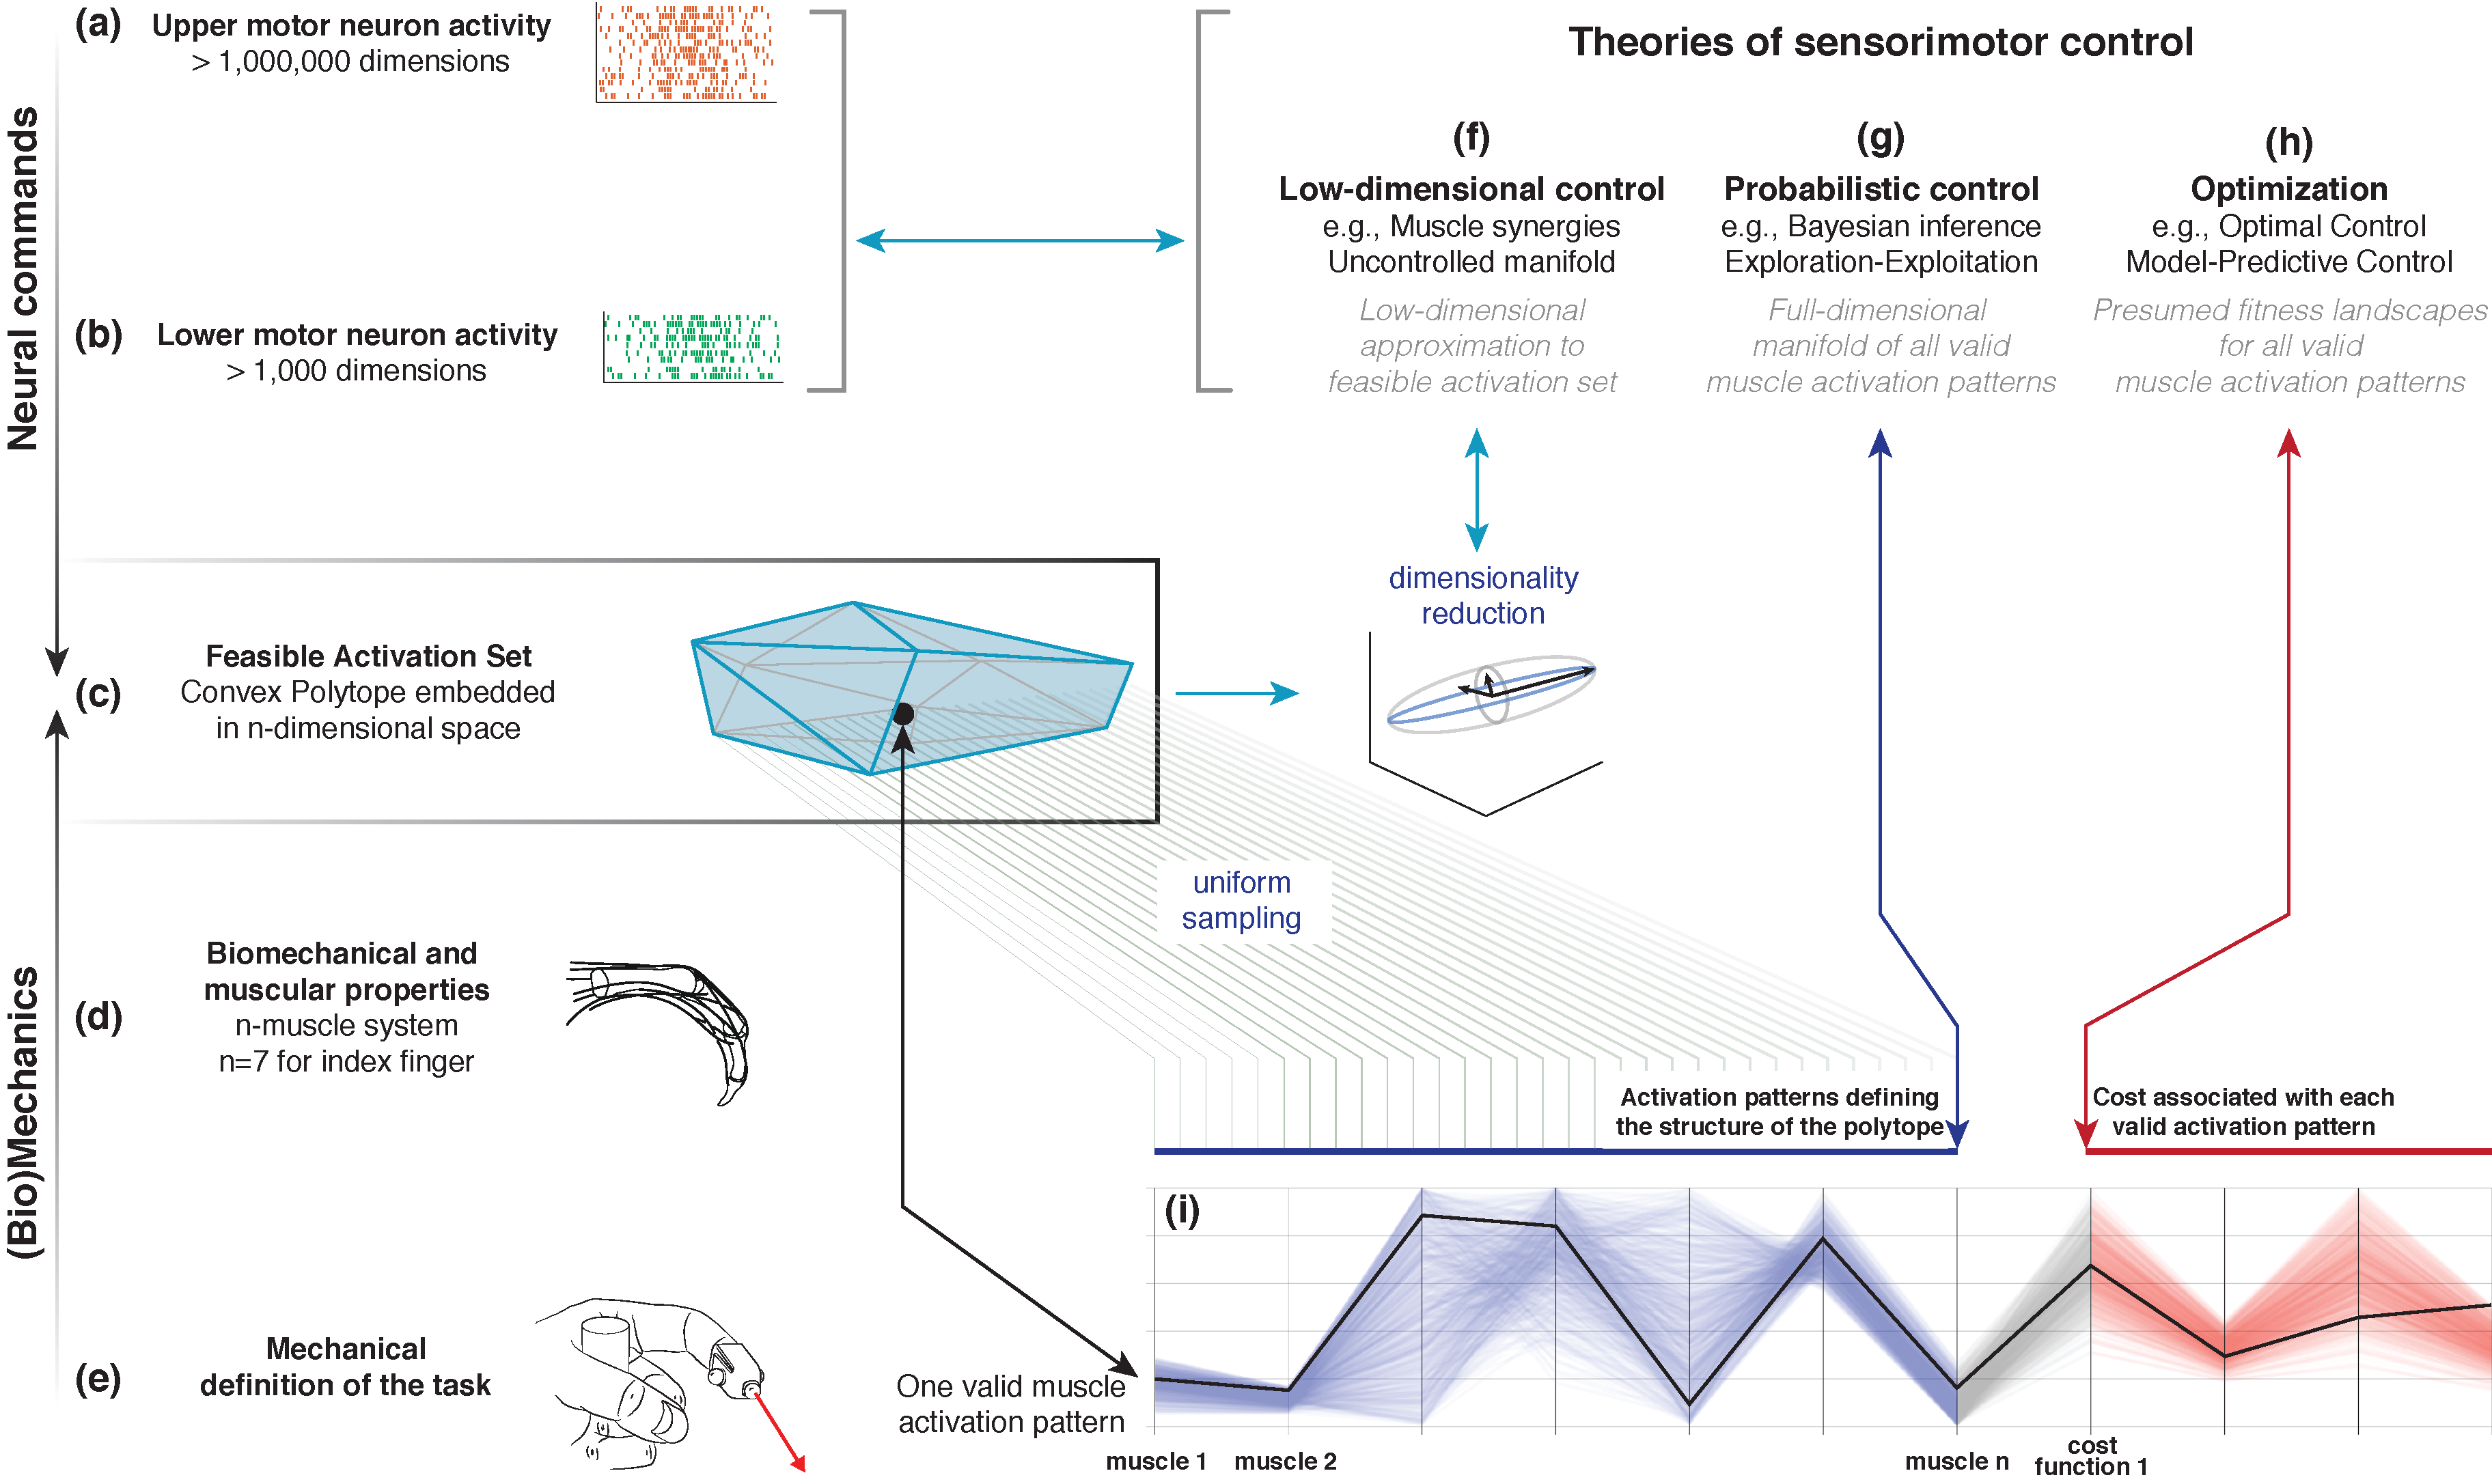
\includegraphics[width=17.2cm]{numbered_figures/figure_1_overview.pdf}
\caption{\textbf{Feasible activation spaces guiding sensorimotor control of a task.} The descending motor command for a given task is issued by the primary motor cortex (a), which projects onto $alpha$-motor neuron pools in the spinal cord (b). The combined drive to all $alpha$-motor neurons of a muscle can be considered its total muscle activation level (a value between 0 and 1). If we consider that motor commands are sent to multiple independently controlled muscles, then the overall motor command can be conceptualized as a multi-dimensional \emph{muscle activation pattern} (i.e., a point) in a high-dimensional \emph{muscle activation space}~\cite{Chao1978Graphical, spoor1983balancing, Kuo1993Human, Valero-Cuevas1998Large} (c). For that muscle activation pattern to be valid, it has to elicit muscle forces (d) capable of satisfying the mechanical requirements of the task---in this case a well directed fingertip force (e). Given the large number of muscles in vertebrates, there is muscle redundancy; there is a large number of valid muscle activation patterns that can produce a given task. We propose that our novel ability to characterize the high-dimensional structure of feasible activation spaces (i) allows to us to compare, contrast and reconcile today's three dominant approaches to redundancy in sensorimotor control (f, g, h).}
\label{fig:overview}
\end{figure*}


The most the nervous system can do, therefore, is select a specific muscle activation pattern from within the feasible activation space---as muscle activation patterns outside of this space are, by definition, inappropriate for the task.
In fact, the feasible activation space defines the landscape upon which all neuromuscular learning and performance must occur.
Understanding neuromuscular control is, therefore, equivalent to understanding how the nervous system finds, explores, inhabits, and exploits the structure of feasible activation spaces~\cite{kutch2012challenges,steele2013number,bizzi2013neural,gallego2017neuron,dingwell2010walkingvariability,racz2013spatiotemporal,steele2015consequences}.

%using dimensionality to say it is a big problem
But the `curse of dimensionality`~\cite{bellman1958dynamic,bellman2015adaptive,avis1992Pivoting} makes it computationally challenging to calculate, describe, and understand the nature and structure of high-dimensional feasible activation spaces~\cite{valero2009computational,Chao1978Graphical,spoor1983balancing,Kuo1993Human,theodorou2010optimalityEMBC,scholz1999uncontrolled,dingwell2010walkingvariability}—even for an isolated human finger or cat leg generating everyday static forces~\cite{kutch2012challenges,Valero-Cuevas2015high-dimensional,valero-cuevas2015fundamentals,sohn2013cat_bounding_box}. This is due to the computational complexity of algorithms applied upon high dimensional spaces.

%the gap
Current theories of neuromuscular control are alternative responses to the curse of dimensionality, which at times can be seem as competing, rather than complementary. However, the fundamental neuromechanics of the limb and the physics of the task are the common ground for all theories. Thus, understanding the nature and structure of feasible activation spaces would help compare, contrast and combine these alternative approaches to neuromuscular control.

%our contribution
We now propose a conceptual and computational framework to provide complete characterizations of feasible activation spaces, thereby contextualizing and unifying multiple theories of neuromuscular control.
As an example, we leverage prior work~\cite{Valero-Cuevas1998Large,kutch2012challenges,Venkadesan2008Neural} to now describe the structure of the feasible activation space for the seven muscles of the index finger when producing static fingertip force. This is the type of fingertip force observed when, for example, pressing hard on a table without finger movement, and is also referred to as an isometric force task.
In this case, the feasible activation space is a polytope embedded in 7-dimensional muscle activation space. A polytope is the name given to bounded convex polyhedra in dimensions higher than 3. Our computational approach hinges on the efficient sampling and complete representation of the structure of high-dimensional polytopes.
This then characterizes all valid muscle activation patterns.
These computational techniques can scale up to $\sim$40 dimensions, which suffices to analyze the neural control of all muscles in a extant vertebrate limb systems.
By providing a complete characterization of all muscle activation patterns for a given motor task, we are able to compare, contrast, combine---and reconcile---today's three dominant approaches to neuromuscular control.
%%%%%%%%%%%%%%%%%%%%%%%%%%%%%%%%%%%%%%%%%%%%%%%%%%%%%%%%%%%%%%%%%%%%%%%%%%%%%%%%%%%%%%%%%%%%%%%%%%%%%%%%


\section*{Results}

The goal of this work is to use different perspectives to describe the high-dimensional structure of these feasible activation spaces; we then show how these spaces allow us to unify today’s theories of neuromuscular control. We used our realistic index finger model to calculate the feasible activation space for the task of producing static fingertip force in the distal direction (see Fig.~\ref{fig:overview}). The model represents each muscle's contribution to fingertip force as a directed force vector at the fingertip; there are 7 of these force vectors at the index fingertip.
As described briefly in the Methods, Hit-and-Run is a method in polytope sampling that we use to sample from the infinite number of muscle activations within the feasible activation space. In effect, given a fingertip task force and the maximum linear fingertip forces each muscle creates, we can collect the muscle activations required to produce that task. As we can now collect thousands of muscle activation patterns for any isometric force task, we examined how the feasible activation spaces (and their representations) change with increasing task intensity in the distal direction (Fig.~\ref{fig:overview}e).

We collected points for multiple task intensities between $0\%$ (i.e., pure co-contraction without output force) and $100\%$ of maximal static force.


\subsection*{Parallel coordinate visualization naturally reveals the structure of the feasible activation space}


\begin{figure}[htbp]
 \centering
 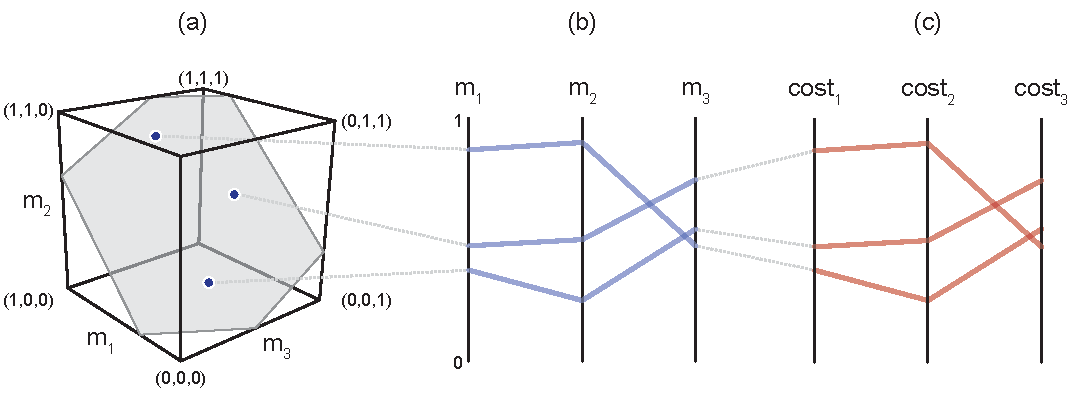
\includegraphics[width=4cm]{numbered_figures/figure_3_parcoord_schematic.pdf}
 \caption{\textbf{Characterizing the high-dimensional structure of a feasible activation space via parallel coordinates.} Consider three points (i.e., muscle activation patterns in Supplemental Fig.~\ref{fig:figure_2_hit_and_run_steps}e) from the feasible activation space (a). The activation level for each muscle (i.e., the coordinates of each point) are sewn across three vertical parallel axes (b). As is common when evaluating multiple valid coordination patterns, each point can be assigned a cost as per an assumed \emph{cost function}. The associated cost for each muscle activation pattern can also be shown as an additional dimension. We show three representative cost functions (c). Activation levels are bound between $0$ and $1$, and costs are normalized to their respective observed ranges.}
 \label{fig:points_to_parcoords_mapping}
\end{figure}

\begin{figure}[htbp]
 \centering
 \includegraphics[width=0.4\textwidth]{numbered_figures/figure_4_parcoord_saturation_edited.png}
 \caption{\textbf{Activation patterns of the seven muscles of the index finger across six magnitudes of a fingertip force} The connectivity across parallel coordinates shows how muscle activation patterns are related in multiple ways to produce a fingertip force vector between 0 (a) to 100\% (f) of maximal magnitude. At these extremes we have, respectively, the coordination patterns that produce pure co-contraction and the one unique solution for maximal output. In between, we see the how the structure of the feasible activation spaces changes as redundancy is lost. In blue are the activation values, and in red are normalized costs for four cost functions common in the literature. \textit{FDP: flexor digitorum profundus, FDS: flexor digitorum superficialis, EIP: extensor indicis proprious, EDC: extensor digitorum communis, LUM: lumbrical, DI: dorsal interosseous, PI: palmar interosseous.}}
 \label{fig:figure_4_parcoord}
\end{figure}

We used Hit-and-Run to sample from feasible activation spaces for 6 task intensities, labeled as task intensities $\alpha$ of $0.0, 0.2, 0.4., 0.6, 0.8$ and $1.0$.
For each task intensity, we ran 100,000 Hit-and-Run iterations and down-sampled to every $100^{th}$ point to produce 1,000 points that are (in our experiments) uncorrelated and uniformly distributed in $P$.
Recall that approaching $100\%$ of maximal force shrinks $P$ to a single, unique solution~\cite{Valero-Cuevas1998Large
}.




Parallel coordinate visualization effectively reveals correlations that exist among the 1,000 valid muscle activation patterns for each magnitude of desired fingertip force, and activation pattern cost, Fig.~\ref{fig:points_to_parcoords_mapping} and Fig.~\ref{fig:figure_4_parcoord}.


An interactive parallel coordinate visualization plot can be accessed at \texttt{https://briancohn.github.io/space-parcoords/}. This interactive interface for parallel coordinate visualization allows us to explore subsets of the valid muscle activation patterns.

For example, restricting the range of muscle activation of one or more muscles shows us the necessary activation levels of the remaining muscles.
This can be used to, say, simulate a 40\% reduction in possible activation to some muscles (e.g., due to a peripheral neuropathy) in the extrinsic extensor muscles of the index finger innervated by the radial nerve (EIP and EDC)~\cite{valero2000quantification}.

\begin{figure}[p]
 \centering
 \includegraphics[width=0.4\textwidth]{supplemental_figures/parcoord_supplemental.pdf}
 \caption{\textbf{Supplemental Figure: Posthoc constraints on a task intensity of 80\%} Here we show four unique examples of constraints applied to the points collected from the feasible activation space. With this, we can rapidly predict how index finger control must change in the event of weakness in specific muscles. We also can see how many points remain once the constraints are added—signaling how the structure of the feasible force space is affected.}
  \label{fig:parcoord_supplemental}
\end{figure}

Figures in the Supplemental Material show how, for 80\% of task intensity (i.e., 80\% of maximal force output), only 29\% (i.e., $\frac{290}{1,000}$) of all possible solutions survive when capping the maximal excitation of EIP and EDC at 60\%. Thus, any neural or muscle dysfunction that compromises the ability of the extensor muscles will limit the choices the nervous system has to produce this force---even at sub-maximal levels. These results further challenge the notion of muscle redundancy as discussed in detail in~\cite{kutch2011muscle,valero-cuevas2015fundamentals}.

Moreover, this same case of task intensity of 80\% and maximal excitation of EIP $\le$60\% reveals important and counterintuitive consequences in the control of musculature. For example, the range of feasible activation level for some muscles do not change too much (FPD, FDS, and LUM), but does change for others (DI and PI). Most interestingly, the range of costs across valid solutions remains broad.

Similarly, we can describe any subset of muscle activation patterns associated with specific ranges for a given cost function. Figures in the Supplemental Material also show how can characterize all muscle activation patterns associated with the lowest 10\% of L2 weighted costs. The coordination patterns that meet this strict criterion are quite different from one another (note the broad ranges and criss-cross patterns).

These relationships among all valid 7-dimensional muscle activations patterns reveal important aspects of the structure of the feasible activation space, and its associated cost landscapes. We see one muscle can affect other muscles in different ways: while limiting PI to 20\% of maximal activation eliminates 30.1\% of the valid solutions, limiting DI to 20\% eliminates 42.8\% of them. Similarly we can distinguish between changes in the extreme values of muscle activation from changes in the number of valid solutions. Consider the range of activation for DI and PI at task intensity of 80\% which lies between 0 and 0.52 and 0.39, respectively. Limiting DI to 20\% pulls PI’s maximum down by nearly 0.20, and the converse has nearly the same effect. However, in both cases, the median activation among surviving solutions changes no more than 0.06. This emphasizes that understanding feasible activation spaces requires and understanding of its internal density and not just its bounds. The density of \textbf{between-muscle} connectivity is seen directly by the density of the lines connecting the different muscles and cost functions. The \textbf{within-muscle} density can be computed by binning points at each activation level value.

Lastly, those same connecting lines in the parallel coordinate visualization allow us to characterize the interrelatedness of valid solutions in 7-dimensional space. For example, the lines connecting FDP and FDS are mostly parallel, indicating a strong positive correlation. In fact, looking at these lines allows one to directly see and understand the Pearson product-moment correlation coefficients of 0.99, -0.50, and -0.06 in the adjacent muscle pairs FDP—FDS, LUM—DI, and EIP—EDC, respectively. The interactive parallel coordinate visualization also allows for any pairwise comparison by simply dragging and reordering the vertical axes---and hovering over individual data rows highlight an individual valid activation pattern atop all others.


\subsection*{Low-dimensional approximations to the feasible activation space}

We applied PCA (Principal Component Analysis) to the valid muscle activation patterns sampled uniformly at random from the feasible activation space. We show results for 10 levels of task intensity. However, we did this in an iterative fashion to replicate the fact that experimental studies can only collect a finite amount of data from each subjects. Thus, from the total pool of 10,000 sub-sampled points sampled by Hit-and-Run (i.e., accepting every 100th point from 100,000 total samples to remove potential autocorrelation among points); sample sizes of 10, 100, and 1,000 points (i.e., simulated `experimental' sample sizes) were replicated 100 times each. We applied PCA to each set of sampled points.

The variance explained by PC1 and PC2 (and its boxplot distribution) for all iterations are shown to change with task intensity for all sample sizes (Fig.~\ref{fig:pca_variance_explained}). Explaining about 13-15\% of the variance, PC3 is exactly equal to the remaining variance not explained by the first two components---this is a result of the feasible activation space being a 3-dimensional polytope $P$ by construction (i.e., recall that 4 task constraints applied to 7 muscles produce a 3-dimensional polytope embedded in the 7-dimensional muscle activation space).

\begin{figure}[htbp]
\centering
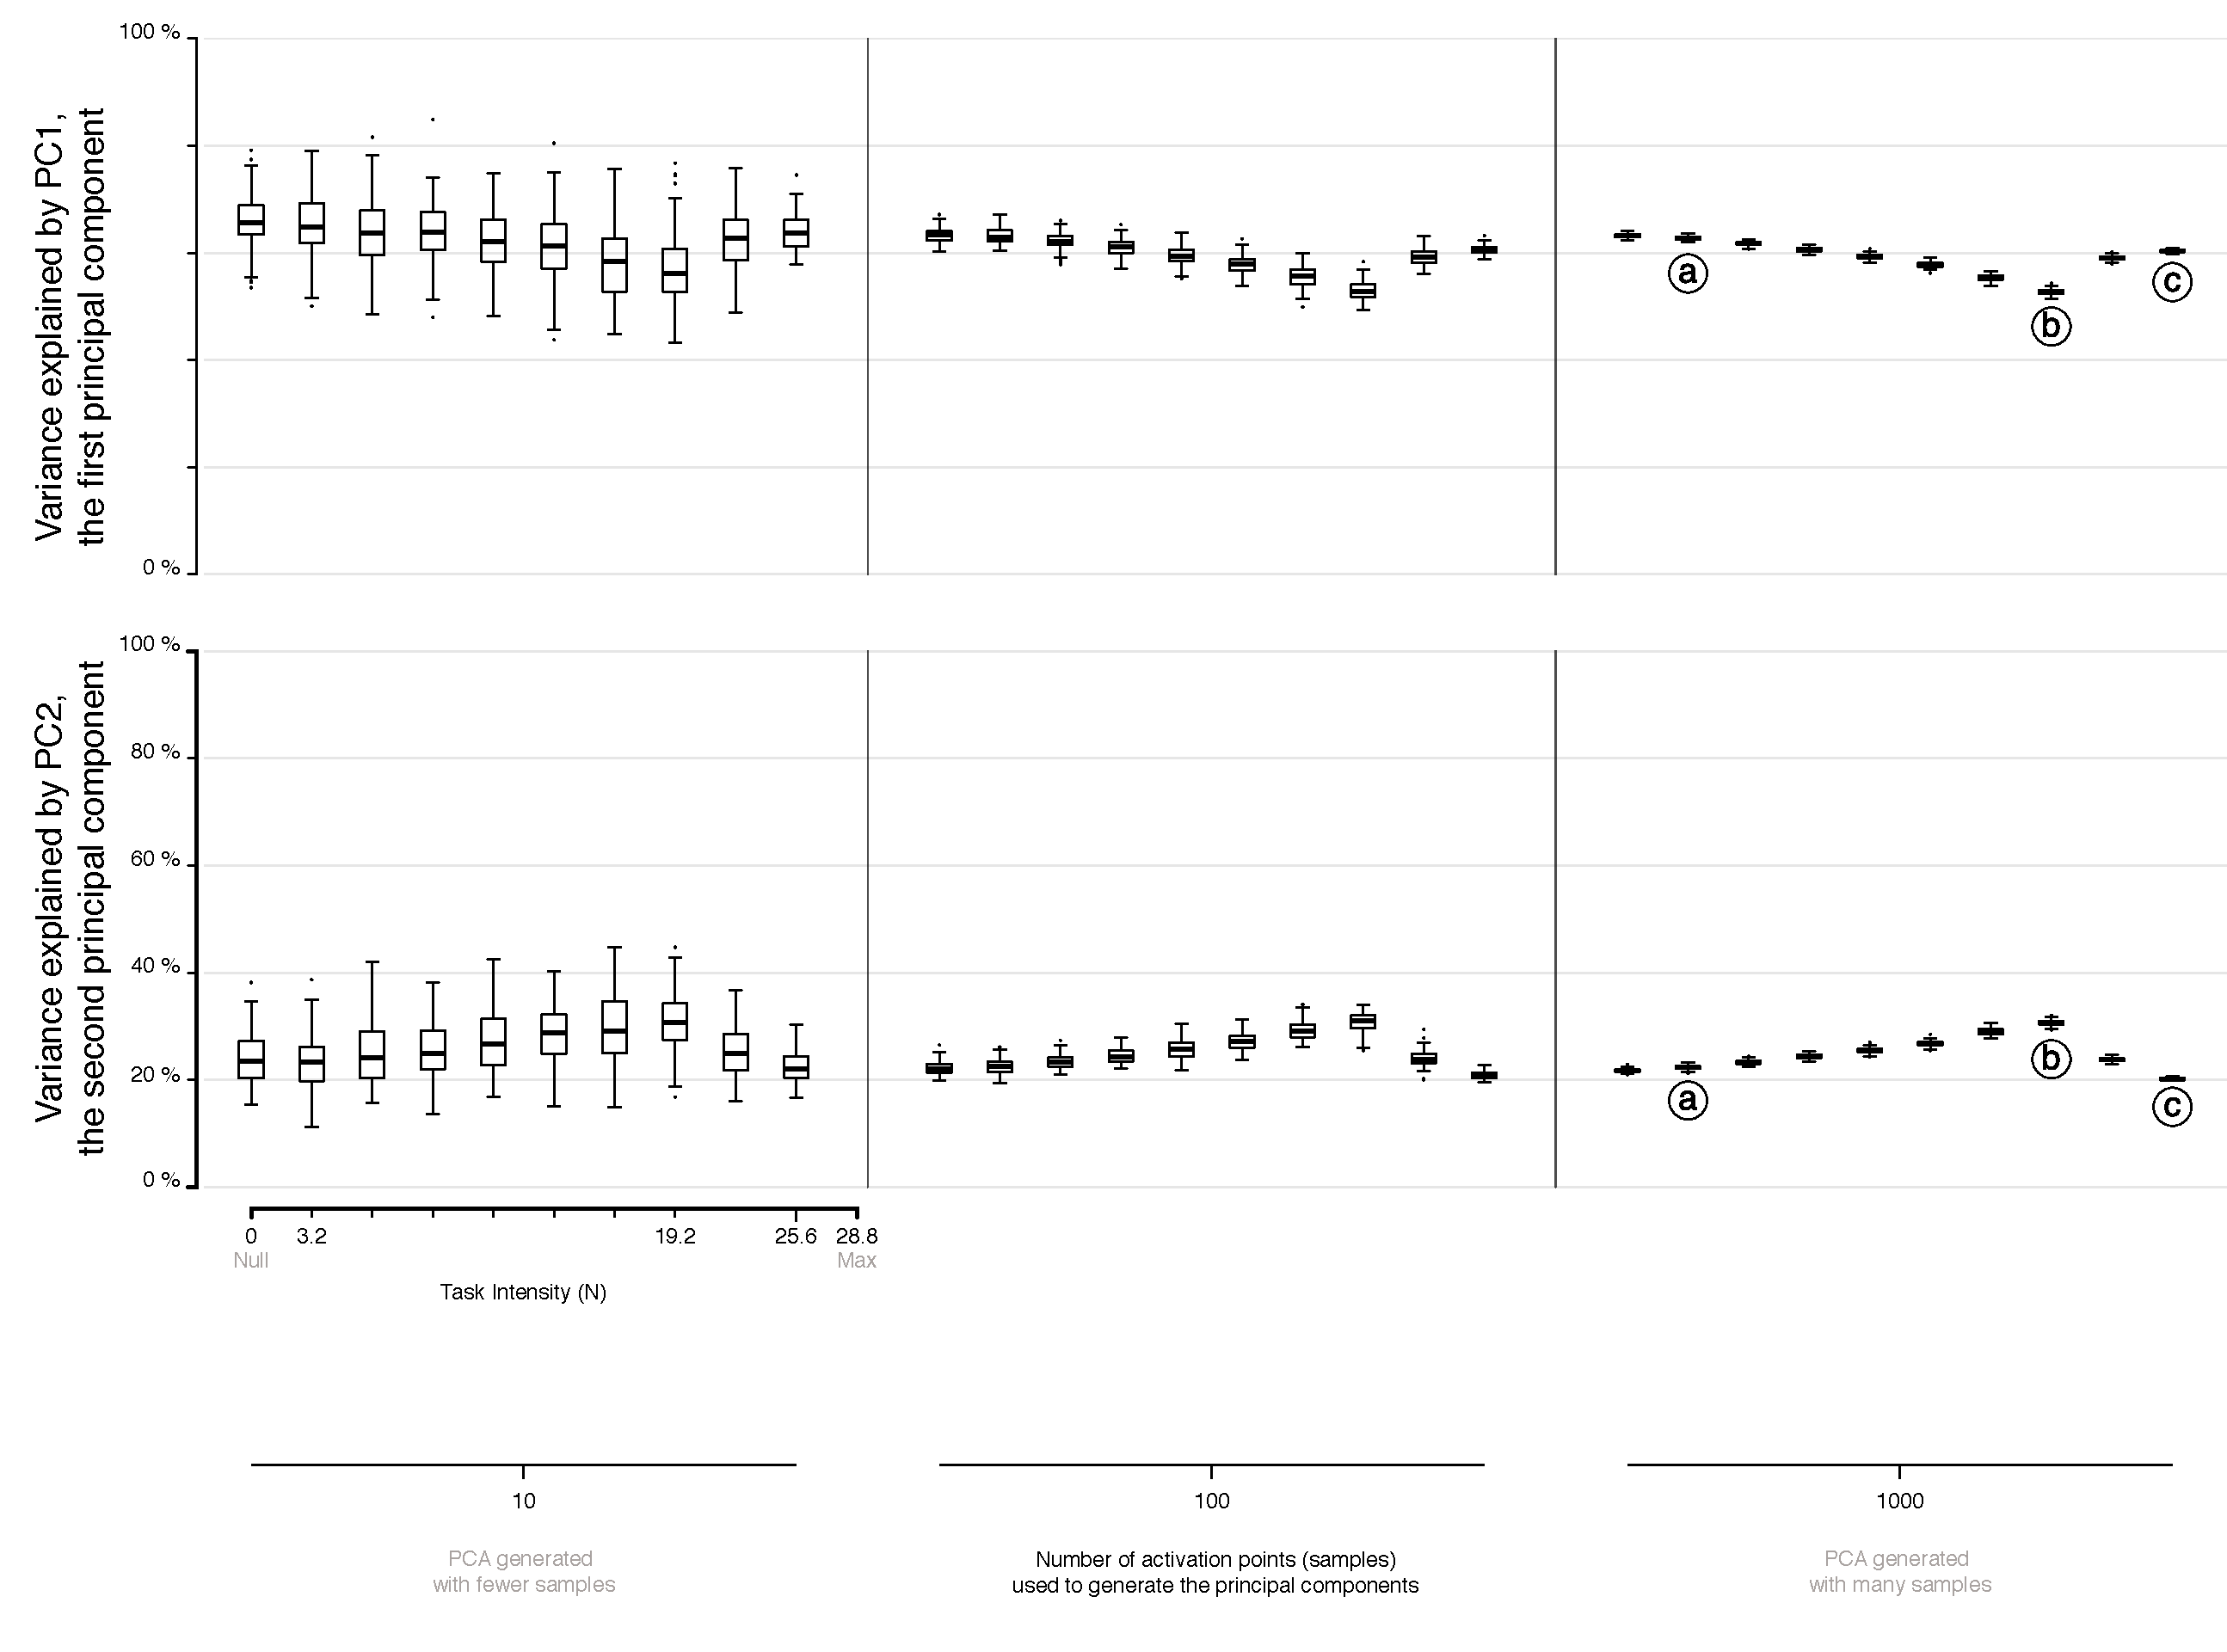
\includegraphics[width=0.4\textwidth]{numbered_figures/figure_7_pca_variance_explained.pdf}
\caption{\textbf{Approximating the structure of feasible activation spaces via principal components analysis (PCA) is sensitive to both the number of points used and the intensity of the task.} Rows show the variance explained by the first (top) and second (bottom) principal components with increasing data points (left to right). It is not possible to generalize the variance explained across tasks intensities, and large numbers of points (i.e., $>$ 100) are needed to confidently estimate the real changes in variance explained as a function of task intensity (cf. points labeled a, b, c).}
\label{fig:pca_variance_explained}

\end{figure}

The boxplots in Fig.~\ref{fig:pca_variance_explained} quantify how different amounts of data change the estimates of variance explained by PC1 and PC2 with task intensity (c.f. labels a vs. b vs. c). We see this dispersion is small in the center and right columns.
Note that the ratio of variance explained between PC1 and PC2 between 50 to 80\% of task intensity is indicative of changes in the aspect ratio of the feasible activation space---which we see changes with task intensity.

Importantly, using experimentally realistic samples sizes of 10 repetitions per subject (leftmost column) not only does not capture this change, but its standard deviation is large enough to blur the statistically significant differences that are known to appear with larger (but experimentally unrealistic) sample sizes.
The impact of impoverishing the number of samples fed to PCA reminds us that inadequate amounts of data obfuscate the underlying changes in the structure of the data analyzed (Fig.~\ref{fig:pca_variance_explained}).

There were also important changes in the loadings of the PC1 and PC2 vectors. While the ratio of variance explained between PC1 and PC2 gives a sense of the aspect ratio of the feasible activation space, the loadings of PC1 and PC2 speak to its orientation.
Fig.~\ref{fig:pca_loadings_detail} shows how the loadings of the PC1 and PC2 vectors change across labels a, b, and c (Fig.~\ref{fig:pca_variance_explained}) corresponding to 11, 66 and 88\% of task intensity, respectively.
What these loadings indicate are the direction in 7-dimensional space, which changes dramatically.

These changes we see in (i) the lower and upper bounds of activations, and in (ii) the relative variance explained and (iii) loadings for PC1 and PC2, demonstrate that the size, shape and orientation of the feasible activation space changes with task intensity. Moreover, these changes represent the best-case scenario given the absence of experimental noise, within- and across-subject variability, and measurement error.


\begin{figure}[htbp]
\centering
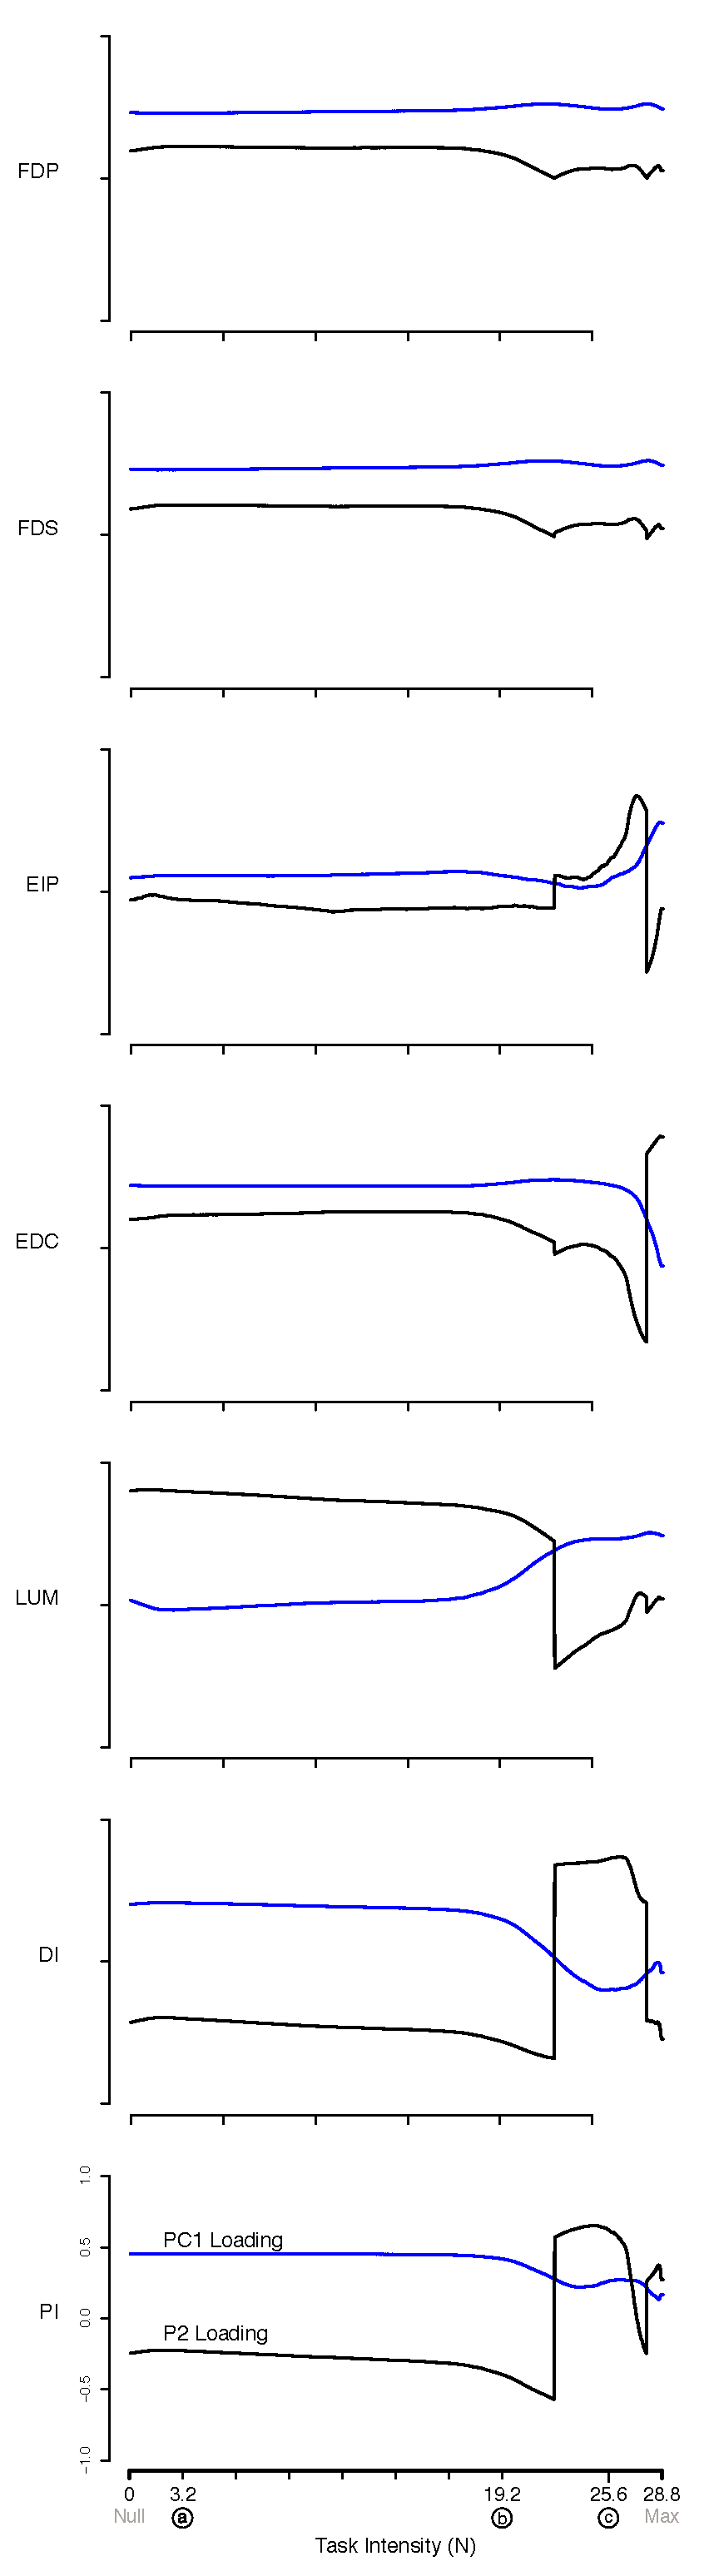
\includegraphics[height=11.2cm]{supplemental_figures/pc_loadings_FDP_made_positive.pdf}
\caption{\textbf{PCA loadings change dramatically as task intensity increases} For each of 1,000 task intensities, we collected 1,000 points from the feasible activation space, and computed three principal components.
Note that the signs of the loadings depend on the numerics of the PCA algorithm, and are subject to arbitrary flips in sign---thus for clarity we plot them such that FDP's loadings in PC1 are positive at all task intensities.
Synergies at representative task intensities a, b, c in Fig.~\ref{fig:pca_variance_explained} differ. This reflects changes in the geometric structure of the feasible activation space as redundancy is lost.}
\label{fig:pca_loadings_detail}
\end{figure}


\subsection*{Changes in the probabilistic structure of the feasible activation space with increasing task intensity, or how muscle redundancy is lost}
The maximal static fingertip force vector in a given direction is produced by a single and unique combination of muscle activations. In contrast, any sub-maximal magnitude of that same vector is produced by an infinite number of solutions~\cite{spoor1983balancing,Chao1978Graphical,valero-cuevas2015fundamentals,Valero-Cuevas2000Predictive}.
Our analysis of feasible activation spaces at different task intensities allows us to characterize how this redundancy changes and is lost.
The histogram heatmaps in Fig.~\ref{fig:figure_6_histogram_heatmap} illustrate the changes and shrinking of within-muscle density of valid activation levels for sub-maximal forces, converging to a single solution for maximal force output. These surface plots show how the normalized histograms (of 1,000 valid activation levels for each muscle) change at each of 100 levels of task intensity between 0 and 1. Following a muscle’s column from bottom to top shows the activation histograms for each magnitude of distal force and ending, naturally, with a spike about the unique value at maximal force production.

\begin{figure*}[htb]
\centering
\includegraphics[width=17.8cm]{numbered_figures/figure_6_histogram_surfaces_v2.pdf}
\caption{\textbf{The within-muscle probabilistic structure of feasible muscle patterns across 1,000 levels of fingertip task intensity.} The changes in the breadth and height for each muscle reveal muscle-specific consequences of task intensity on their probability distributions. The cross-section of each density plot is the 50-bin histogram of activation for each muscle, at that task intensity. Height represents the percentage of solutions for that task. The axis going into the page indicates increasing fingertip task intensity up to 100\% of maximal. Color is used to provide perspective.}
\label{fig:figure_6_histogram_heatmap}
\end{figure*}


The flat areas in each surface plot (e.g. clearly visible for DI) represent muscle activation levels that are not valid for that task intensity. That is, there exist no valid muscle activation patterns that contain that muscle at that level, and thus no points are found there.

These plots show the nature and rate of convergence to the unique solution for maximal force output across muscles.
We find that the histograms of activation levels for each muscle need not be symmetric, nor have the same shape (skewness and kurtosis) as the magnitude of the output force increases.
For some muscles the convergence accelerates after 60\% or 80\% of task intensity (as in LUM and EIP), while others converge monotonically along the entire progression (e.g. DI and PI).
The peaks (i.e. modes) of each histogram at each task intensity represents the slice of the polytope that has the largest relative volume along that muscle dimension (i.e., greatest frequency of that level of muscle activation across all valid solutions). Importantly, for most muscles (FDP, FDS, EIP, EDC, and LUM), the mode is not necessarily located at the same relative level of activation needed for maximal force output. That is, the histogram at high levels of force is not simply a shifted version of the histogram at low levels of force. The histograms for DI are the exception, whose modes seems to scale linearly with task intensity.

%bounding box representation
These histograms, in conjunction with the results in the parallel coordinate visualization, also demonstrate that the structure of feasible activation spaces cannot be inferred from their bounding boxes alone (i.e., upper and lower activation bounds for each muscle).
An immediate example is how, for most task intensities, both EIP and LUM have similar lower and upper bounds near 0 and 1, respectively---yet their distributions are thoroughly distinct.

%%%%%%%%%%%%%%%%%%%%%%%%%%%%%%%%%%%%%%%%%%%%%%%%%%%%%%%%%%%%%%%%%%%%%%%%%%%%%%%%%%%%%%%%%%%%%%%%%%%%%%%%
\section*{Discussion}
\subsection*{Summary}

Feasibility theory, as a conceptual and computational approach, is a means to pierce the curse of dimensionality to establish a physics-based ground truth for neuromuscular control. This practical approach can now characterize---in a complete way---the set of all valid ways to activate multiple muscles to produce a given task.
Feasible activation spaces are, in fact, \emph{the} neuromechanical landscapes upon which all neuromuscular learning, control, and performance must occur. Therefore, we provide an integrative and unifying perspective that demonstrates how today's dominant theories of neuromuscular control are alternative approximations to feasible activation spaces from optimization, geometric, and probabilistic perspectives.

\subsection*{The value of a cost function}

Optimization is the oldest computational approach to finding valid muscle activation patterns that produce limb function (e.g.,~\cite{Chao1978Graphical}).
While optimization is a reasonable hypotheses to explore neuromuscular control~\cite{todorov2002optimal}, some criticize it as mathematical abstraction that anthropomorphizes neurons with the ability to choose, evaluate and follow cost functions in high-dimensions~\cite{deRugy2012habitual,loeb2012optimal}.
There is an intimate relationship between optimization and feasible activation spaces~\cite{chvatal1983linear}. Optimization is analogous to finding a best solution in the dark---guided by repeated evaluations of a cost-function. Computing the feasible activation space is then a means to `turn on the lights' to see all possible valid solutions independently of cost~\cite{valero-cuevas2015fundamentals}. Our complete sampling of high-dimensional feasible activation spaces ~\cite{smith1984efficient,lovasz1999hit} allows us to compare and contrast \emph{families} of solutions instead of \emph{individual} optimal solutions for a particular cost function.
Fig.~\ref{fig:figure_4_parcoord} demonstrates a complete description of families of valid coordination patterns and their relationship to alternative costs. Importantly, similar valid muscle activation patterns can have dissimilar costs, and vice versa.

Because these explorations can be done for alternative cost functions, they can provide quantitative overall descriptions of high-dimensional `cost landscapes.'
By not having to insist on (or settle for) individual optimal---or near-optimal---solutions, we now have the same ability the nervous system has to explore, compare and contrast multiple valid ways to coordinate muscles. Importantly, the relationships among valid muscle activation patterns emerge naturally from the physical properties of the limb and definition of the task. This  cost-agnostic approach allows us to re-evaluate our assumptions about what the nervous system cares---and does not care---about. Lastly, this cost-agnostic approach also provides a powerful tool for inverse optimization, i.e., uncovering latent cost functions from data~\cite{tsirakos1997inverse}. Our comparison across cost functions using parallel coordinates is already a form of inverse optimization.

\subsection*{Structure, correlation, and synergies}

The physical properties of the limb and definition of the task also define a low-dimensional structure of the feasible activation space \cite{valero-cuevas2015fundamentals}. Therefore, it is expected that experimental recordings of muscle activations during limb function will exhibit a dimensionality that is smaller than the number of muscles~\cite{kutch2012challenges,alessandro2013musclesynergies}. Thus, applying PCA to the points sampled from the feasible activation space also finds that few PCs can explain the variance in the data.

This application of PCA at increasing task intensities (i.e., as muscle redundancy is lost) allows us to demonstrate---for the first time to our knowledge---several important features and limitations of dimensionality reduction. For example, we see that the aspect ratio (Fig.~\ref{fig:pca_variance_explained}) and orientation (Fig.~\ref{fig:pca_loadings_detail}) of the feasible activation spaces change as their size shrinks (Fig.~\ref{fig:figure_6_histogram_heatmap}).
Thus, such \emph{descriptive} synergies extracted from limited experimental observations likely do not generalize well across task intensities.
It is important to distinguish \emph{descriptive} synergies (the dominant approach in the literature to extract synergies from experimental data using dimensionality reduction techniques such as PCA) from \emph{prescriptive} synergies (those  known to be implemented by the controller)~\cite{valero-cuevas2015fundamentals}.

This also has important consequences to motor control and learning. Producing force vectors at the endpoint of a finger or limb with accurate magnitude and direction are critical for versatile manipulation and locomotion~\cite{cole2006age,valero1998large,donelan2004mechanical}. If a given synergy can produce such accurate force vectors only for a given task intensity (and thus inaccurate ones at other intensities), then the attractiveness of synergies to simplify the neuromuscular control of the limb is reduced.
%That is, if a synergy for low task intensity is used for other intensities, they will produce an inaccurate finger or limb force.
To compensate, the nervous system would need to learn, recall and implement specific synergies for each force level. In prior experimental work, we have shown that the nervous system produces accurate fingertip forces of different magnitudes by, instead, likely scaling a remembered muscle activation pattern to produce forces of different magnitudes, together with a full-dimensional, real-time error correction neural controller~\cite{Valero-Cuevas2000Scaling}. Note that interpreting this experimental result still as a synergy-based approach would defeat the purpose of synergies as a means to simplify the control by reducing its dimensionality.

Our results also show how experiments with realistically moderate numbers of participants and test trials likely do not contain sufficient data to produce robust estimates of descriptive synergies across task intensities. As per the curse of dimensionality, sampling uniformly at random from high-dimensional spaces is exponentially difficult. Thus, even for this anatomically complete 7-muscle finger model, PCA depends strongly on the number of independent observations, such as uncorrelated trials from one subject or different subjects. Figure~\ref{fig:pca_variance_explained} shows that 100 to 1,000 such ideal data points from a simulated `test subject ' are needed to produce accurate estimates of changes in PC1 and PC2 with task intensity (c.f. labels a vs. b vs. c). Future studies should explore how many experimental data points are sufficient from a given subject when recording from only a subset of the many (20+) muscles of human limbs in the presence of experimental noise, inherent stochasticity of EMG, and within- and between-subject variability. Some studies have begun to ask subjects to explore different ways to perform a given task \cite{berger2014effective} (i.e., estimate the structure of the feasible activation space), but in practice such studies cannot likely collect sufficient data uniformly at random to obtain accurate estimates of the descriptive synergies~\cite{kutch2012challenges}. While our results suggest caution when interpreting synergies obtained experimentally, we underscore that dimensionality-reduction is a useful approach to capture global geometric properties of feasible activation spaces.

\subsection*{Toward probabilistic neuromuscular control}

Our results are particularly empowering for the emerging field of probabilistic neuromuscular control~\cite{kording2004bayesian, Kording2014130,berniker2013examination,sanger2011distributed }. Suppose that the nervous system uses some form of probabilistic or Bayesian learning and control strategy. Such approach requires two enabling---and biologically feasible---elements: \emph{trial-and-error iterative exploration}, and \emph{ memory-based exploitation} of the probability density functions used to approximate the feasible activation spaces~\cite{kording2004bayesian}. The parallel coordinate plots and histograms in Fig.~\ref{fig:points_to_parcoords_mapping} and \ref{fig:figure_6_histogram_heatmap} provide, to our knowledge, the first complete~\cite{smith1984efficient,lovasz1999hit} characterization of such multi-dimensional joint probability density functions for a realistic tendon-driven system performing a well-defined task.

These techniques and results now empower the study of fundamental aspects of probabilistic control. For example, an organism can only execute so many trial-and-error iterations during learning, likely too few to completely and exhaustively sample the high-dimensional feasible space of interest. This makes it much more likely that, by virtue of being more easily found, an organism will find and preferentially exploit the strong modes (i.e., narrow and high peaks in Figs.~\ref{fig:figure_4_parcoord}, \ref{fig:parcoord_supplemental}, and \ref{fig:figure_6_histogram_heatmap}) of the multi-dimensional probability density functions than any other region of feasible activation spaces. Thus, first, the maximal ranges of feasible activations described by the bounding box \cite{sohn2013cat_bounding_box,Valero-Cuevas2015high-dimensional} may have little practical bearing on how those tasks are learned and executed. And second, those same strong modes would represent strong attractors to create and reinforce motor habits. Habitual control has been proposed based on experimental and empirical data as an alternative to a strict optimization approach to neuromuscular control~\cite{deRugy2012habitual}. Our work now provides the computational means to link habitual to probabilistic control. This allows us to generate testable hypotheses of how these motor habits are defined by the structure of the feasible activation space, how they are learned by the organism, and how difficult or easy it is to break out of them.

Thus, motor learning likely needs to proceed from adopting easily-found solutions independently of their cost, to using some low dimensional approximation to the gradient of the cost landscape, to then transitioning to less likely but potentially less costly subregions of the solutions space. This integrative perspective leads us to propose a hybrid approach to motor learning and execution where the practical limits on trial-and-error iterations are coupled with the low-dimensional structure of the solution space to enable some form of heuristic local optimization to create sub-optimal motor habits. Importantly, the organism performs strict optimization or synergy control at its peril. Take, for example, the case of a 2-dimensional feasible activation space embedded in 3-D, Fig.~\ref{fig:figure_2_hit_and_run_steps}e. Taking a step from any one valid point to another valid point on the plane runs the risk of `falling off' the solution space and failing at the task---a risk that is exponentially exacerbated in higher-dimensions. Thus, improvements in the neighborhood of a good solution necessarily risk task failure and potential injury. These are all arguments in support of the evolutionary and developmentally useful strategy to use good-enough control based on habit or sensorimotor memory rather than optimization~\cite{deRugy2012habitual, santello2012context}. This may explain why mass practice and coaches are so critical to achieve elite athletic performance~\cite{gladwell2008outliers}.

\subsection*{Clinical implications}
This line of thinking has consequences to neurorehabilitation. Neurological conditions disrupt feasible activation spaces, be it by affecting anatomy of the limb, muscle strength and independence with which muscles can be controlled. Functional recovery following the disruption, if not destruction, of the landscape of valid muscle activation patterns requires re-learning existent, or building new, probability density functions. This occurs just when older adults suffer from reduced perceptuo-motor learning rates \cite{coats201450scliff}.

A probabilistic landscape for neuromuscular function begins to explain why neurorehabilitation in aging adults is so difficult (e.g., ~\cite{hardwick2016motor}) and why motor learning in children takes thousands of repetitions~\cite{adolph2012thousands}---while also generating new rehabilitation strategies, and testable hypotheses around them, that leverage knowledge of the nature and structure of feasible activation spaces.
%%%%%%%%%%%%%%%%%%%%%%%%%%%%%%%%%%%%%%%%%%%%%%%%%%%%%%%%%%%%%%%%%%%%%%%%%%%%%%%%

\subsection*{Author Affiliations}

Include department, institution, and complete address, with the ZIP/postal code, for each author. Use lower case letters to match authors with institutions, as shown in the example. Authors with an ORCID ID may supply this information at submission.

\subsection*{Submitting Manuscripts}

All authors must submit their articles at \href{http://www.pnascentral.org/cgi-bin/main.plex}{PNAScentral}. If you are using Overleaf to write your article, you can use the ``Submit to PNAS'' option in the top bar of the editor window.

\subsection*{Format}

Many authors find it useful to organize their manuscripts with the following order of sections;  Title, Author Affiliation, Keywords, Abstract, Significance Statement, Results, Discussion, Materials and methods, Acknowledgments, and References. Other orders and headings are permitted.

\subsection*{Manuscript Length}

PNAS generally uses a two-column format averaging 67 characters, including spaces, per line. The maximum length of a Direct Submission research article is six pages and a PNAS PLUS research article is ten pages including all text, spaces, and the number of characters displaced by figures, tables, and equations.  When submitting tables, figures, and/or equations in addition to text, keep the text for your manuscript under 39,000 characters (including spaces) for Direct Submissions and 72,000 characters (including spaces) for PNAS PLUS.

\subsection*{References}

References should be cited in numerical order as they appear in text; this will be done automatically via bibtex, e.g. \cite{belkin2002using} and \cite{berard1994embedding,coifman2005geometric}. All references, including for the SI, should be included in the main manuscript file. References appearing in both sections should not be duplicated.  SI references included in tables should be included with the main reference section.

\subsection*{Data Archival}

PNAS must be able to archive the data essential to a published article. Where such archiving is not possible, deposition of data in public databases, such as GenBank, ArrayExpress, Protein Data Bank, Unidata, and others outlined in the Information for Authors, is acceptable.

\subsection*{Language-Editing Services}
Prior to submission, authors who believe their manuscripts would benefit from professional editing are encouraged to use a language-editing service (see list at www.pnas.org/site/authors/language-editing.xhtml). PNAS does not take responsibility for or endorse these services, and their use has no bearing on acceptance of a manuscript for publication.

\subsection*{Digital Figures}
\label{sec:figures}

Only TIFF, EPS, and high-resolution PDF for Mac or PC are allowed for figures that will appear in the main text, and images must be final size. Authors may submit U3D or PRC files for 3D images; these must be accompanied by 2D representations in TIFF, EPS, or high-resolution PDF format.  Color images must be in RGB (red, green, blue) mode. Include the font files for any text.

Figures and Tables should be labelled and referenced in the standard way using the \verb|\label{}| and \verb|\ref{}| commands.

Figure \ref{fig:frog} shows an example of how to insert a column-wide figure. To insert a figure wider than one column, please use the \verb|\begin{figure*}...\end{figure*}| environment. Figures wider than one column should be sized to 11.4 cm or 17.8 cm wide.

\subsection*{Single column equations}

Authors may use 1- or 2-column equations in their article, according to their preference.

To allow an equation to span both columns, options are to use the \verb|\begin{figure*}...\end{figure*}| environment mentioned above for figures, or to use the \verb|\begin{widetext}...\end{widetext}| environment as shown in equation \ref{eqn:example} below.

Please note that this option may run into problems with floats and footnotes, as mentioned in the \href{http://texdoc.net/pkg/cuted}{cuted package documentation}. In the case of problems with footnotes, it may be possible to correct the situation using commands \verb|\footnotemark| and \verb|\footnotetext|.

%% Do not use widetext if paper is in single column.
\begin{widetext}
\begin{align*}
(x+y)^3&=(x+y)(x+y)^2\\
       &=(x+y)(x^2+2xy+y^2) \numberthis \label{eqn:example} \\
       &=x^3+3x^2y+3xy^3+x^3.
\end{align*}
\end{widetext}

\begin{table}%[tbhp]
\centering
\caption{Comparison of the fitted potential energy surfaces and ab initio benchmark electronic energy calculations}
\begin{tabular}{lrrr}
Species & CBS & CV & G3 \\
\midrule
1. Acetaldehyde & 0.0 & 0.0 & 0.0 \\
2. Vinyl alcohol & 9.1 & 9.6 & 13.5 \\
3. Hydroxyethylidene & 50.8 & 51.2 & 54.0\\
\bottomrule
\end{tabular}

\addtabletext{nomenclature for the TSs refers to the numbered species in the table.}
\end{table}

\subsection*{Supporting Information (SI)}

The main text of the paper must stand on its own without the SI. Refer to SI in the manuscript at an appropriate point in the text. Number supporting figures and tables starting with S1, S2, etc. Authors are limited to no more than 10 SI files, not including movie files. Authors who place detailed materials and methods in SI must provide sufficient detail in the main text methods to enable a reader to follow the logic of the procedures and results and also must reference the online methods. If a paper is fundamentally a study of a new method or technique, then the methods must be described completely in the main text. Because PNAS edits SI and composes it into a single PDF, authors must provide the following file formats only.

\subsubsection*{SI Text}

Supply Word, RTF, or LaTeX files (LaTeX files must be accompanied by a PDF with the same file name for visual reference).

\subsubsection*{SI Figures}

Provide a brief legend for each supporting figure after the supporting text. Provide figure images in TIFF, EPS, high-resolution PDF, JPEG, or GIF format; figures may not be embedded in manuscript text. When saving TIFF files, use only LZW compression; do not use JPEG compression. Do not save figure numbers, legends, or author names as part of the image. Composite figures must be pre-assembled.

\subsubsection*{3D Figures}

Supply a composable U3D or PRC file so that it may be edited and composed. Authors may submit a PDF file but please note it will be published in raw format and will not be edited or composed.

\subsubsection*{SI Tables}

Supply Word, RTF, or LaTeX files (LaTeX files must be accompanied by a PDF with the same file name for visual reference); include only one table per file. Do not use tabs or spaces to separate columns in Word tables.

\subsubsection*{SI Datasets}

Supply Excel (.xls), RTF, or PDF files. This file type will be published in raw format and will not be edited or composed.

\subsubsection*{SI Movies}

Supply Audio Video Interleave (avi), Quicktime (mov), Windows Media (wmv), animated GIF (gif), or MPEG files and submit a brief legend for each movie in a Word or RTF file. All movies should be submitted at the desired reproduction size and length. Movies should be no more than 10 MB in size.

\subsubsection*{Still images}

Authors must provide a still image from each video file. Supply TIFF, EPS, high-resolution PDF, JPEG, or GIF files.

\subsubsection*{Appendices}

PNAS prefers that authors submit individual source files to ensure readability. If this is not possible, supply a single PDF file that contains all of the SI associated with the paper. This file type will be published in raw format and will not be edited or composed.

\matmethods{
The methods to obtain feasible activation spaces for `tendon-driven' limbs are described in detail in the textbook \emph{Fundamentals of Neuromechanics} and references therein~\cite{valero-cuevas2015fundamentals}. This tendon-driven approach explicitly and distinctly avoids the conceptual approach to combine multiple muscle actions into net torques at each joint. Rather, it emphasizes studying the individual actions of all muscles at all levels of analysis, from their neural activation to their contributions to fingertip force. We describe them briefly here.
\label{s:methods}
\subsection*{Theory}
Consider a tendon-driven limb, such as a finger, with $n$ independently controllable muscles, where we define the neural command to each muscle as a positive value of activation between 0 (no activation) and 1 (maximal activation).
We can then visualize the set of all feasible neural commands (i.e., all possible muscle activation patterns) as the points contained in a positive n-dimensional cube with sides of length equal to 1. A specific muscle activation pattern is a \emph{point} (i.e., an n-dimensional vector $\textbf{a}$) in this n-dimensional cube~\cite{Chao1978Graphical, spoor1983balancing, Kuo1993Human, Valero-Cuevas1998Large}.
Now consider a specific task, such as producing a vector of static force with the fingertip, as when holding an object. Clearly, not all muscle activation patterns inside the n-dimensional cube can produce that desired static fingertip force vector: bone lengths, kinematic degrees of freedon, anatomical routing, posture, and muscle strength inequities define the subset of points in the n-cube can produce a fingertip force vector of a specific magnitude and direction.
As described in~\cite{Chao1978Graphical, spoor1983balancing, Kuo1993Human, valero-cuevas2015fundamentals} the musculoskeletal anatomy of the limb, the need to control individual tendons, and the physics of a motor task uniquely specify a polytope embedded in $\mathbb{R}^n$ (i.e., the feasible activation space). This polytope contains the family of (potentially infinite) valid muscle activation patterns that can produce this static force production task.
However, these valid muscle coordination patterns are not arbitrarily different because, by construction, the geometric structure of the polytope that contains them defines strict spatial correlations among them~\cite{kutch2012challenges}.

\paragraph*{System of linear equations to simulate static force production by a tendon-driven system}

Consider producing a vector of static force with the endpoint of the limb in a given posture. The constraints that define that task (i.e., the direction and magnitude of the force vector at the endpoint) are linear equations~\cite{valero-cuevas2015fundamentals} that come from the mapping between neural activation of individual muscles to static endpoint forces and torques the limb can produce. This mapping is linearly modeled by the equation
\begin{align}
\label{eq:constraints}
		 \begin{pmatrix}
f_{x}\\
f_{y}\\
f_{z}\\
\tau_{x}\\
\tau_{y}\\
\tau_{z}
\end{pmatrix}=\textbf{w} = H\textbf{a} = H\begin{pmatrix}
a_{1}\\
a_{2}\\
a_{3}\\
...\\
a_{n}
\end{pmatrix}
, \textbf{a} \in [0,1]^n
\end{align}
where $H$ is the matrix of linear constraints defined by the musculoskeletal anatomy of the limb~\cite{Valero-Cuevas2015high-dimensional}, \textbf{a} is the input vector of $n$ muscle activations, $\textbf{f} \in \mathbb{R}^m$ is the m-dimensional limb output `wrench' (i.e., the forces and torques the finger can produce at the endpoint).

The output wrench, $m$, is at most 6-dimensional (i.e., 3 forces and 3 torques) depending on the number of kinematic degrees of freedom of the limb, and usually $m < n$ because limbs have more muscles than kinematic degrees of freedom~\cite{valero-cuevas2015fundamentals}. Muscles can only pull, so elements of \textbf{a} cannot be negative, and are capped at 1 (i.e., 100\% of maximal muscle activation).

What are the muscle coordination patterns that produce a given task? As explained in~\cite{valero-cuevas2015fundamentals}, the task of producing a static fingertip force vector is defined by specifying the desired values for the elements of the endpoint forces and torques of $\textbf{w}$. Each such constraint equation defines a hyperplane of dimension $n-1$, and their combination defines the task completely. The \emph{feasible activation space} of the task, if it is well posed~\cite{chvatal1983linear}, is defined by the points $\textbf{a}$ that lie within the $n$-cube and at the intersection of all constraint hyperplanes.

Geometrically speaking, the feasible activation space is a $(n-m)$-dimensional convex polytope $P$ embedded in $\mathbb{R}^n$ that contains all n-dimensional muscle coordination patterns (i.e., points $\textbf{a}$) that satisfy all constraints, and therefore can produce the task. Increasing task specificity by adding more constraints naturally decreases the dimensionality and changes the size and shape of the feasible activation space~\cite{Kuo1993Human,sohn2013cat_bounding_box,inouye2016muscle}.


\paragraph*{The Hit-and-Run algorithm uniformly samples from feasible activation spaces}
\label{ss:hitrun}

Calculating the geometric properties of convex polytopes in high dimensions is computationally challenging. Taking the generalized concept of an $n$-dimensional volume as an example of a geometric property of interest, the exact volume computations for n-dimensional polytopes is known to be tractable only in a polynomial amount of time (i.e., $\#P$-hard)~\cite{Dyer}.
Currently available volume algorithms can only handle polytopes embedded in small dimensions like 10 or slightly more~\cite{Bueler2}. Studying vertebrate limbs in general, however, can require including several dozen muscles, such as our studies of a 17-muscle human arm and a 31-muscle cat hindlimb model~\cite{Valero-Cuevas2015high-dimensional}; and other limb models have over 40 muscles such as~\cite{arnold2010model, kutch2012challenges, hamner2010muscle, de2014human}.

Similar difficulties arise when computing other geometric properties such as the shape and aspect ratio of $P$ in high dimensions. We and others have described polytopes $P$ by their bounding box (i..e, the range of values in every dimension)~\cite{sohn2013cat_bounding_box,kutch2011muscle}, but that singularly overestimates the shape and volume of the feasible activation space as discussed in~\cite{Valero-Cuevas2015high-dimensional}.
Take Fig.~\ref{fig:figure_2_hit_and_run_steps}e as an example, where the bounding box of the 2-dimensional polygon has a volume---even though a plane has zero volume---, and can be almost as large as the positive unit cube itself. Similar problems arise in the interpretation of the inscribed and circumscribed ball~\cite{inouye2014optimizing}.

We applied the Hit-and-Run method to sample points from the feasible activation space—a method that is evaluated and justified in ~\cite{valero-cuevas2015fundamentals, YYY_IEEE_STR}.
This complete probabilistic method describes the structure of feasible activation spaces $P$ with a set of uniformly-at-random muscle activation patterns that produce the same wrench. This enables us to derive descriptive statistics, histograms, and point densities of the set of valid muscle activation patterns $\textbf{a}$ uniformly sampled from the polytope. To do so, we use the Hit-and-Run method. We have presented a detailed explanation of the theory (In Chapter X of \cite{YYY_FUNDAMENTALS_BOOK}), have justified the utility of this method on tendon-driven models of the index finger \cite{YYY_IEEE_STR}.

\subsection*{Example of a tendon-driven system}
\paragraph*{Realistic 3-D model of a 7-muscle human index finger}
\label{ss:finger}
We applied this methodology to our published model of an index finger for static fingertip force production.
The model is described in detail elsewhere~\cite{valero-cuevas2009computational}.
Briefly, the input to the model is a 7-D muscle activation pattern $\textbf{a}$, and the output is a 4-D wrench (i.e., static forces and torque) at the fingertip $\textbf{w}$

\begin{eqnarray}
\textbf{w} = H \textbf{a} \\
H=J^{-T}RF_o \\
H \in \mathbb{R}^{4 \times 7}
\end{eqnarray}

where

\begin{equation}
\label{eq:a}
\textbf{a}=
\begin{pmatrix}
a_{FDP}\\
a_{FDS}\\
a_{EIP}\\
a_{EDC}\\
a_{LUM}\\
a_{DI}\\
a_{PI}
\end{pmatrix}
\end{equation}

In Cartesian coordinates, the 4-dimensional output wrench corresponds to the anatomical directions shown in Fig.~\ref{fig:overview}e.

\begin{equation}
\label{eq:wc}
\textbf{w}=
\begin{pmatrix}
f_{x}\\
f_{y}\\
f_{z}\\
\tau_{x}
\end{pmatrix} =
\begin{pmatrix}
f_{radial}\\
f_{distal}\\
f_{palmar}\\
\tau_{radial}
\end{pmatrix}
\end{equation}




The biomechanical model $H$ includes three serial links articulated by four kinematic degrees of freedom (ad-abduction, flexion-extension at the metacarpophalangeal joint, and flexion-extension at the proximal and distal interphalangeal joints). The action of each of the seven muscles (FDP: \emph{flexor digitorum profundus}, FDS: \emph{flexor digitorum superficialis}, EIP: \emph{extensor indicis proprius}, EDC: \emph{extensor digitorum communis}, LUM: \emph{lumbrical}, DI: \emph{dorsal interosseous}, and PI: \emph{palmar interosseous}) on each joint to produce torque is given by the moment arm matrix $R \in \mathbb{R}^{4 \times 7}$. Lastly, $J \in \mathbb{R}^{4 \times 4}$ and $F_0 \in \mathbb{R}^{7 \times 7}$ are the Jacobian of the fingertip with 4 kinematic degrees of freedom, and the diagonal matrix containing the maximal strengths of the seven muscles, respectively~\cite{valero-cuevas2015fundamentals,Valero-Cuevas2000Scaling}. The finger posture was defined to be $0^\circ$ ad-abduction and $45^\circ$ flexion at the metacarpophalangeal joint, and $45^\circ$ and $10^\circ$ flexion, respectively, at the proximal and distal interphalangeal joints.

\paragraph*{Feasible activation space for a static fingertip force task}

Our goal is to find the family of all feasible muscle activation patterns that can produce a given task. In particular, the task we explored is producing various magnitudes of a submaximal static force in the distal direction $f_{distal}$ --- in the absence of any $\tau_{radial}$, shown in Fig.~\ref{fig:overview}f. Therefore the feasible activation space is a polytope $P$ in 7-dimensional activation space that meets the following \emph{four} linear constraints in $\textbf{a}$~\cite{Valero-Cuevas1998Large,valero-cuevas2015fundamentals,Valero-Cuevas2000Scaling}

\begin{eqnarray}
f_{radial} = 0 \\
f_{distal} = \emph{desired magnitude as \% of maximal} \\
f_{palmar} = 0 \\
\tau_{palmar} = 0
\end{eqnarray}

These four constraints on the static output of the finger yield a 3-dimensional (i.e., $7-4=3$) polytope $P$ embedded in 7-dimensional activation space.
For details on how to create such models, apply task constraints and find such polytopes via vertex enumeration methods, see~\cite{valero-cuevas2015fundamentals}.

Thus all valid output wrenches will have the form

\begin{equation}
\label{eq:wrench}
\textbf{w}=
\begin{pmatrix}
0\\
\text{Desired distal task intensity in N} \\
0\\
0
\end{pmatrix}
\end{equation}

For the index finger model used in this paper, the published maximal feasible force in the distal direction is 28.81 Newtons. We defined the normalized desired distal task intensity as a value ranging between $0$ and $1$, i.e., each submaximal force can be produced by any of the points contained in its corresponding feasible activation space. For the production of a maximal force with $\alpha=1$ the feasible activation space shrinks to a single point~\cite{spoor1983balancing,Chao1978Graphical,chvatal1983linear,Valero-Cuevas2000Scaling}.

\subsection*{Analysis of feasible activation spaces}
\paragraph*{Parallel coordinates visualization shows the location of all points across all dimensions}

Parallel coordinates are a common graphical approach to visualize interactions among high-dimensional data, which has been used in biomechanical studies~\cite{bachynskyi2013biomechanical, krekel2010visual}.
To demonstrate this visualization method, consider the results of the simple 3-dimensional example shown in Fig.~\ref{fig:figure_2_hit_and_run_steps}e. We begin by drawing $n$ parallel vertical lines for each of the dimensions $n$ (i.e., 3 muscles).
With the axis limits of each line set between 0 and 1, each point (Fig.~\ref{fig:points_to_parcoords_mapping}a) is then represented by connecting their coordinates by $n-1$ lines as shown in Fig.~\ref{fig:points_to_parcoords_mapping}b.

\paragraph*{Neural and metabolic cost functions}

As mentioned in the Introduction, the field of neuromuscular control has a long historical tradition of using optimization to find muscle activation patterns that minimize effort, which requires the (often contentious) definition of cost functions~\cite{spoor1983balancing,Chao1978Graphical,Prilutsky2000Muscle,crowninshield1981physiologically}. Therefore, we used four representative cost functions to calculate the relative fitness of each of the muscle activation patterns sampled---in effect also calculating the fitness landscape across all possible solutions. The cost functions are defined at the level of neural effort ($L_1$, and $L_2$ norms); and at the level of metabolic cost, thought to be approximated by neural drive weighted by the strength of each muscle ($L_1^w$ and $L_2^w$ norms)~\cite{Prilutsky2000Muscle,crowninshield1981physiologically}.

To visualize the costs associated with each valid muscle coordination pattern, we simply added four vertical lines at the far right of the parallel coordinates plot, one for each cost function, Fig.~\ref{fig:points_to_parcoords_mapping}c. The variables $a_i$ and $F_{0i}$ represent the activation of the $i^{th}$ muscle in a given muscle activation pattern, and the maximal strength of each muscle~\cite{Prilutsky2000Muscle,crowninshield1981physiologically}. Maximal muscle strengths are approximated by the multiplying each muscle's physiological cross-sectional area, in $cm^2$, by the maximal active muscle stress of mammalian muscle, $35~N/{cm^2}$~\cite{Zajac1993Muscle}. These four cost functions are but four examples as the literature contains many others as any investigator is in fact free to chose any cost function deemed relevant to their study.


\paragraph*{Histograms of the activation level of each muscle across all valid solutions}

Muscle-by-muscle histograms are another straightforward way to visualize the many points sampled from the convex polytope. Histograms are particularly helpful because they are approximations to probability density functions.
They visualize the relative number of solutions (i.e., density of solutions) that required a particular level of activation from a particular muscle within its range of $[0,1]$.
In addition, the upper and lower bounds of the histograms show, in fact, the size of the side of the bounding box of the polytope in every dimension (i.e., for independently controlled muscle).

\paragraph*{Dimensionality reduction}

Investigators have repeatedly reported that electromyographical signals (i.e, experimental estimates of muscle activation patterns) tend to exhibit strong correlations with one another.
In these experimental descriptions of dimensionality reduction of neuromuscular control, only few independent functions---sometimes called synergies---suffice to explain the majority of the variability in the observed muscle activation patterns~\cite{kutch2012challenges,steele2013number,bizzi2013neural,dingwell2010walkingvariability,steele2015consequences,alessandro2013musclesynergies,krishnamoorthy2003muscle}.
Principal components analysis (PCA) is a widely used technique to extract these few independent basis functions (correlation vectors called principal components, PCs) from high-dimensional data~\cite{Clewley2008Estimating}.
In this case, PCs are often called the experimental representations of synergies of neural origin~\cite{kutch2012challenges}.

Therefore, we also applied PCA to points (i.e., muscle coordination patterns) sampled from the feasible activation space at each force level.
This provides the PCs that describe the correlations among valid muscle activation patterns for a given task.
For example, the feasible activation space $P$ in Fig.~\ref{fig:figure_2_hit_and_run_steps}e is a 2-dimensional polygon embedded in 3-dimensional activation space. Thus, applying PCA to points sampled from the polygon will extract 2 synergies (i.e., 3-dimensional correlation vectors PC1 and PC2) that wholly explain the feasible activation space. By extension, in the case of fingertip force production in Fig.~\ref{fig:overview}, the feasible activation space is a 3-dimensional polytope embedded of the 7-dimensional activation space. And PCA should extract, by construction, as many synergies as there are dimensions in the feasible activation space. For static force production with the index fingertip (i.e., 7 muscles and 4 constraints), we know that 3 principal components should describe 100\% of the variance in points sampled from the feasible activation space (i.e., 7-dimensional correlation vectors PC1, PC2, and PC3).

Applying PCA to our data allows us to test whether and how its results change when applied to feasible activation spaces for different magnitudes of fingertip force. We applied PCA to feasible activation spaces for fingertip task intensities ranging from 0 to 90\% of maximal.
We compare both the variance explained by each PC and their vector direction (i..e, the `loadings' or correlations among muscle~\cite{valero2016robot}) as the force level increases.
Lastly, we tested whether our PCA results are sensitive to the number of points sampled from each feasible activation space. This is important because experimental studies test 10 or so subjects in practice, which may be too few when sampling from high-dimensional spaces.


%%%%%%%%%%%%%%%%%%%%%%%%%%%%%%%%%%%%%%%%%%%%%%%%%%%%%%%%%%%%%%%%%%%%


}

\showmatmethods % Display the Materials and Methods section

\acknow{Research reported in this publication was supported by the National Institute of Arthritis and Musculoskeletal and Skin Diseases of the National Institutes of Health (NIH) under Awards Number R01 AR-050520 and R01 AR-052345 to FVC, and the Swiss National Science Foundation (SNF Project 200021\_150055 / 1) to BG, KF and FVC. The content is solely the responsibility of the authors and does not necessarily represent the official views of the SNSF or the NIH. We thank Komei Fukuda for his integral support in designing this research collaboration. We thank J Pugliesi, T Kim, C Lim, A Baugus, P Vachhani, and A Boling for extending the scientific rigor of this work through reviews, documentation, and code}

\showacknow % Display the acknowledgments section

% \pnasbreak splits and balances the columns before the references.
% If you see unexpected formatting errors, try commenting out this line
% as it can run into problems with floats and footnotes on the final page.
\pnasbreak

% Bibliography
\bibliography{plos_cohn_bibliography}

\end{document}
